\documentclass{beamer}
\usetheme{Hannover}
\setbeamersize{sidebar width left=0pt}
\usepackage[T1, T2A]{fontenc}
\usepackage[utf8]{inputenc}
\usepackage[russian]{babel}
\usepackage{hyperref}
\usepackage{graphicx}
\graphicspath{ {../Images/} }

\author{Григорий Матюхин}
\date{\today}
\title{Лабораторная работа \textnumero8.}
\subtitle{Планировщики событий}

\begin{document}
\begin{frame}[plain]
	\titlepage
\end{frame}
\section{Цель работы}
\begin{frame}[plain]
	\frametitle{Цель работы}
	Получение навыков работы с планировщиками событий \texttt{cron} и \texttt{at}.
\end{frame}

\subsection{Планирование задач с помощью cron}
\begin{frame}[plain]
	\frametitle{Планирование задач с помощью cron}
	Посмотрите статус демона \texttt{crond}:
	\\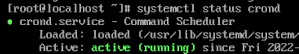
\includegraphics{1.png}
\end{frame}
\begin{frame}[plain]
	Посмотрите содержимое файла конфигурации \texttt{/etc/crontab}:
	Посмотрите список заданий в расписании:
	\\
\includegraphics{2.png}
\end{frame}
\begin{frame}[plain]
	Откройте файл расписания на редактирование. Добавьте следующую строку в файл расписания: \texttt{*/1 * * * * logger This message is written from root cron}:
	\\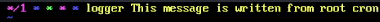
\includegraphics{3.png}
\end{frame}
\begin{frame}[plain]
	Посмотрите список заданий в расписании:
	\\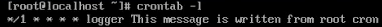
\includegraphics{4.png}
\end{frame}
\begin{frame}[plain]
	Не выключая систему, через некоторое время (2–3 минуты) просмотрите журнал системных событий:
	\\
\includegraphics{5.png}
\end{frame}
\begin{frame}[plain]
	Измените запись в расписании crontab на следующую \texttt{0 */1 * * 1-5 logger This message is written from root cron}:
	\\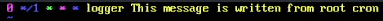
\includegraphics{6.png}
\end{frame}
\begin{frame}[plain]
	Посмотрите список заданий в расписании:
	\\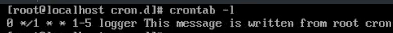
\includegraphics{7.png}
\end{frame}
\begin{frame}[plain]
	Перейдите в каталог \texttt{/etc/cron.hourly} и создайте в нём файл сценария с именем \texttt{eachhour}:
	\\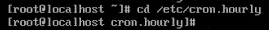
\includegraphics{8.png}
\end{frame}
\begin{frame}[plain, fragile]
	Откройте файл \texttt{eachhour} для редактирования и пропишите в нём следующий скрипт (запись сообщения в системный журнал):
	\begin{verbatim}
#!/bin/sh
logger This message is written at $(date)
  \end{verbatim}

	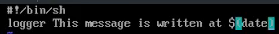
\includegraphics{9.png}
\end{frame}
\begin{frame}[plain]
	Сделайте файл сценария \texttt{eachhour} исполняемым:
	\\
\includegraphics{10.png}
\end{frame}
\begin{frame}[plain]
	Теперь перейдите в каталог \texttt{/etc/crond.d} и создайте в нём файл с расписанием eachhour. Откройте этот файл для редактирования и поместите в него следующее содержимое \texttt{11 * * * * root logger This message is written from /etc/cron.d}:
	\\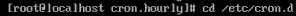
\includegraphics{11.png}
	\\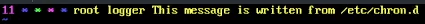
\includegraphics{12.png}
\end{frame}
\begin{frame}[plain]
	Не выключая систему, через некоторое время (2–3 часа) просмотрите журнал системных событий:
	\\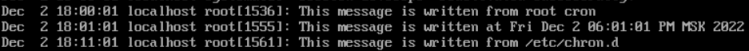
\includegraphics{13.png}
\end{frame}



\subsection{Планирование заданий с помощью at}
\begin{frame}[plain]
	\frametitle{Планирование заданий с помощью at}
	Запустите терминал и получите полномочия администратора:
	Проверьте, что \texttt{служба atd} загружена и включена:
	\\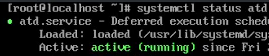
\includegraphics{14.png}
\end{frame}
\begin{frame}[plain]
	Задайте выполнение команды \texttt{logger message from at} в 9:30 (или замените на любое другое время, когда вы работаете над этим упражнением). Для этого введите \texttt{at 9:30}. Затем введите \texttt{logger message from at}:
	\\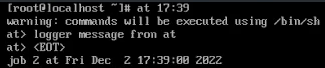
\includegraphics{15.png}
\end{frame}
\begin{frame}[plain]
	Убедитесь, что задание действительно запланировано \texttt{atq}
	\\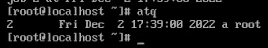
\includegraphics{16.png}
\end{frame}
\begin{frame}[plain]
	Посмотрите, появилось ли соответствующее сообщение в лог-файле в указанное вами время.
	\\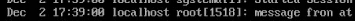
\includegraphics{17.png}
\end{frame}

\section{Вывод}
\begin{frame}[plain]
	\frametitle{Вывод}
	В ходе выполнения данной работы я получил навыков работы с планировщиками событий \texttt{cron} и \texttt{at}.
\end{frame}

\end{document}
